\documentclass[11pt]{article}
\usepackage[utf8]{inputenc} % Para caracteres en espa�ol
\usepackage{amsmath,amsthm,amsfonts,amssymb,amscd}
\usepackage{multirow,booktabs}
\usepackage[table]{xcolor}
\usepackage{fullpage}
\usepackage{lastpage}
\usepackage{enumitem}
\usepackage{multicol}
\usepackage{fancyhdr}
\usepackage{mathrsfs}
\usepackage{wrapfig}
\usepackage{setspace}
\usepackage{esvect}
\usepackage{calc}
\usepackage{multicol}
\usepackage{cancel}
\usepackage{graphicx}
\graphicspath{ {pictures/} }
\usepackage[retainorgcmds]{IEEEtrantools}
\usepackage[margin=3cm]{geometry}
\usepackage{amsmath}
\newlength{\tabcont}
\setlength{\parindent}{0.0in}
\setlength{\parskip}{0.05in}
\usepackage{empheq}
\usepackage{framed}
\usepackage[most]{tcolorbox}
\usepackage{xcolor}
\colorlet{shadecolor}{orange!15}
\parindent 0in
\parskip 12pt
\geometry{margin=1in, headsep=0.25in}
\theoremstyle{definition}
\newtheorem{defn}{Definition}
\newtheorem{reg}{Rule}
\newtheorem{exer}{Exercise}
\newtheorem{note}{Note}
\begin{document}
\setcounter{section}{0}

\thispagestyle{empty}

\begin{center}
{\LARGE \bf Section 1}\\
{\large AE435}\\
Spring 2018
\end{center}
\begin{defn} 
\textbf{Electric Propulsion} - The use of electric power to accelerate propellant for propulsion. 
\end{defn}
\\
\subsection*{Key Concepts:} 
\begin{note} \textbf{Overcome limitations of the Rocket Equation which expresses mission capability in terms of "characteristic velocity" or "Delta-V" $\Delta V$.}\end{note}
\begin{shaded}
\textbf{The Rocket Equation} \newline
\begin{equation*}
\Delta V = c \ln(\frac{M_{o}}{M_{f}})
\end{equation*}
Where:
\begin{equation*}
\begin{split}
c &= \text{Effective Exhaust Velocity} \\
M_{o} &= \text{Initial Mass} \\
M_f &= \text{Final Mass}
\end{split}
\end{equation*}
\end{shaded}
For a \textbf{Chemical Thruster}, the effective exhaust velocity, $c$, is limited by the enthalpy of combustion. In other words, it is limited by the chemical bond energy of the propellant. 
\begin{shaded}
\textbf{Effective Exhaust Velocity for a Chemical Thruster} \newline
\begin{equation*}
c = U_{e} +  \frac{A_{e}}{\dot{m}}(P_{e}-P_{\infty})
\end{equation*}
Where:
\begin{equation*}
\begin{split}
U_{e} &= \text{Exhaust Velocity} \\
A_e &= \text{Exit Area} \\
\dot{m} &= \text{Mass Flow Rate}\\
P_e &= \text{Exit Pressure} \\
P_{\infinity} &= \text{Ambient Pressure (0 in Vacuum)}\\
\end{split}
\end{equation*}
\end{shaded}
For \textbf{Electric Propulsion}, the effective exhaust velocity, $c$, is limited by the power supplied. 
\newpage
\begin{note} \textbf{Electric Propulsion is "Power Limited"}\end{note}
\\
It is difficult to generate power in space (International Space Station \~ 120kW). Power limited means the power of the exhaust beam is limited. In other words
\begin{equation*}
P_{\text{jet}} = \frac{1}{2}\dot{m}c^{2}
\end{equation*}
is limited. Where $P_{\text{jet}}$ is the power in the exhaust beam, the amount of kinetic energy being expelled per unit time.
\begin{itemize}
\item \textbf{Corollary 1:} Power Limited \& High $c$ $\Rightarrow$ Low $\dot{m}$ \& Low Thrust
\item \textbf{Corollary 2:} Low Thrust $\Rightarrow$ Low Acceleration ($10^{-3}$ - $10^{-6}$ g's)
\item \textbf{Corollary 3:} Low Acceleration $\Rightarrow$ Long Trip Times $\Rightarrow$ No Manned Missions
\end{itemize}
\vspace{10mm}
\begin{note} \textbf{For each mission, ($\Delta V$ \& Time) there is an optimum $c$.}\end{note}
\\
It is not the case to say "Lets just do a high $\Delta V$", NO! For each optimum $c$ there is also an optimum thruster. The specific impulse level needed for a mission determines the thruster we choose to use (Ion, Hall, etc.).
\begin{enumerate}
\item Find the $\Delta V$ for mission
\item Find the optimum $c$
\item Pick the "best" thruster.
\end{enumerate}
\newpage
\section{Introduction to Electric Propulsion}
\subsection{Space Propulsion}
See handwritten notes .
\subsection{Comparison of Chemical Propulsion and Electric Propulsion - An Example}
Consider a small 5lb chemical thruster capable of 22N of thrust. From Equation 2, in a vacuum,
\begin{equation*}
\text{Thrust} = \frac{d}{dt}(\text{momentum}) = \dot{m} u_{e} + A_{e}(P_{e}-0) = \dot{m}c 
\end{equation*}
For a hydrazine monopropellant, $I_{SP}$ = 220sec.
\begin{shaded}
\textbf{Specific Impulse}
\begin{equation}
I_{SP} = \frac{\text{impulse}}{\text{propellant weight}} = \frac{\int T dt}{g M_{prop}}
\end{equation}
Where, $g$ is always $9.81 \frac{m}{s^{2}}$
\end{shaded}
For a constant thrust, T, for time $t_t$ and 
\begin{equation}
\dot{m}=\frac{M_{prop}}{t_t}
\end{equation}
then
\begin{equation}
I_{SP} = \frac{T t_t}{g M_{prop}} = \frac{\dot{m}c}{g \dot{m}} = \frac{c}{g}
\end{equation}
\newline \newline
So, $I_{SP}$ = 220sec $\rightarrow$ $c=2156 \frac{\text{m}}{\text{s}}$
\newline
\newline
$\dot{m}$ for 5lb thruster is $\dot{m}=\frac{T}{c} = 0.1\frac{\text{kg}}{\text{s}}$
\\
\begin{shaded}
\textbf{Exhaust Beam Power}
\begin{equation}
P_{\text{jet}} = \frac{1}{2}\dot{m}c^{2} = \frac{1}{2}Tc
\end{equation}
\end{shaded}
\\
Which for our problem equates to $ = 24kW$ which is HUGE! (Space Shuttle produces power in the GW range). The smallest electric propulsion is $<$1W
\newpage
\subsection{Thruster Efficiency}
Recall that thrusters are essentially just energy conversion device. For Electric Propulsion:
\vspace{70mm}
\begin{center}
\textbf{Figure 1}
\end{center}
\textbf{Thruster Efficiency:}
\begin{equation}
\eta_{t}=\frac{\text{Beam Power as Thrust}}{\text{Power to Thruster}} = \frac{\frac{1}{2}Tc}{P_{in}}
\end{equation}
\newline
\newline
\newline
\textbf{Power Processing Unit Efficiency:}
\begin{equation}
\eta_{PPU}=\frac{\text{Power to Thruster}}{\text{Power from Source}}= \frac{P_{in}}{P}
\end{equation}
\newline
\newline
\newline
\textbf{Overall System Efficiency:}
\begin{equation}
\eta_{t}=\frac{\text{Beam Power as Thrust}}{\text{Power from Source}}= \frac{\frac{1}{2}Tc}{P} = \eta_{t}\eta_{PPU}
\end{equation}
\newline
\newline
\newline
The PPU takes the power and puts it in a form the thruster can use. For Electric Propulsion, thruster effieciency ($\eta_t$) ranges from $5\%$ to $90\%$ depending on the thruster.
\begin{itemize}
\item PPT: 0\%-2\%
\item Hall: 50\% - 60\%
\item Ion: 80\%
\end{itemize}
\newpage
\subsection{Thrust Discussion}
What is and isn't a force?
\begin{center}
 \begin{tabular}{||c | c||} 
 \hline
  Fundamental Forces & Caused by... \\ [0.5ex] 
 \hline\hline
 Gravity & Gravitation Field (mass) \\ 
 \hline
Pressure & Particle Momentum/Energy\\ 
 \hline
Shear & Particle Collisions (Viscosity)\\ 
 \hline
Electric Force & E-field (charge)\\ 
 \hline
Magnetic Foce & B-field (charge motion)\\[1ex] 
 \hline
\end{tabular}
\end{center}
There is no force called "Thrust." Thrust is caused by shear and pressure when considering the exhaust of a chemical thruster. For electric propulsion however, we now have thrust caused by all of the fundamental forces listed. Thrust is the resulting effect when other forces push-on/propels a space craft, rocket, gas turbine engine etc.
\newline
\newline
Consider a Control Volume containing a rocket and all exhaust. Apply Newton's Law:
%\vspace{200mm}
\vfill
\\
\begin{center}
\textbf{Figure 2}
\end{center}
\begin{framed}
\textbf{Theory:}
\newline
The change in momentum of mass in the C.V. equals the sum of forces on the C.V. (gravity). If $g=0$, the momentum in the C.V. is constant because it contains all the exhaust.
\end{framed}
\newpage
\begin{shaded}
\textbf{Proof} \newline
Change in $\vv{P}$ (momentum) in time $\Delta t$ as we accelerate to the effective exhaust velocity, c:
\begin{equation*}
\begin{split}
\text{(before): \hspace{10mm}}& \vv{P}(t) = (m+\Delta m)\vv{v} \\
\text{(after): \hspace{10mm}}& \vv{P}(t+\Delta t) = m(\vv{v} + \Delta\vv{v})+\Delta m(\vv{v} + \Delta\vv{v}-\vv{c}) \\
\text{(difference): \hspace{10mm}}& \Delta P = \vv{P}(t+\Delta t) - \vv{P}(t) = m\Delta\vv{v} - \Delta m \vv{c} + \Delta m \Delta \vv{v}
\end{split}
\end{equation*}
\newline
Take the limit, $\Delta t \rightarrow dt$ :
\begin{equation*}
\frac{\Delta P}{dt} = \frac{d\vv{P}}{dt} = m \frac{d\vv{v}}{dt} - \frac{dm}{dt} \vv{c}
\end{equation*}
\newline
Equating $\frac{d\vv{P}}{dt}$ with the gravitational force $\vv{F_{g}}$, we get:
\begin{equation*}
\begin{split}
m \frac{d\vv{v}}{dt} - \frac{dm}{dt} \vv{c} = F_{g} \qquad
\text{or}
\qquad
m\vv{\dot{v}} = F_{g} + \dot{m} \vv{c}
\end{split}
\end{equation*}
Where:
\begin{equation*}
\begin{split}
m\vv{\dot{v}} &= \text{Change in Rocket Momentum} \\
F_{g} &= \text{Gravity Causes Rocket Momentum Change} \\
\dot{m} \vv{c} &= \text{Rate of Increase of Exhaust Momentum}\\
\end{split}
\end{equation*}
\end{shaded}
Note that the third term in the equation $m\vv{\dot{v}} = F_{g} + \dot{m} \vv{c}$ has units of force but is not actual a force. This we call Thrust! $c$, comes from the fundamental forces initially discussed. We will develop models to predict what these forces will be on a certain Electric Thruster and use those to predict the thrust on an Electric Propulsion device. 
\newline
\newline
Some points to be made on the "after" equation $\vv{P}(t+\Delta t) = m(\vv{v} + \Delta\vv{v})+\Delta m(\vv{v} + \Delta\vv{v}-\vv{c})$
are:
\begin{equation*}
\begin{split}
\vv{v} + \Delta\vv{v} &= \text{Some change because we expelled some small amount of mass in exhaust.} \\
-\vv{c} &= \text{This is negative because the rocket and the exhaust are going in opposite directions.}\\
\end{split}
\end{equation*}
\newline \newline
To emphasize its importance, we highlight the following equation explained above.
\begin{framed}
\begin{equation}
m\vv{\dot{v}} = F_{g} + \dot{m} \vv{c}
\end{equation}
\end{framed}
\newpage
\subsection{Thrust-to-Power $\frac{T}{P}$ $[\frac{N}{W}]$}
The Thrust-to-Power ratio is an important space craft design parameter.
\\
\begin{equation*}
\begin{split}
\frac{T}{P} = \frac{2\eta}{c} \propto \frac{1}{c} \qquad \text{and}\qquad \frac{T}{P} \propto \frac{1}{I_{SP}}
\end{split}
\end{equation*}
With the overall efficiency equation from Section 1.3 and with Equation 3 from Section 1.2 shown above we can achieve an equation for the Thrust-to-Power ratio.
\vspace{5mm}
\begin{exer}
\textbf{
\\
For Electric Propulsion with $\eta = 0.5$ and $I_{SP} = 1000\text{sec}$, find the Thrust-to-Power ratio.}
\newline \newline
\begin{equation*}
\frac{T}{P} = 10^{-4} \frac{\text{N}}{\text{W}}  \text{\qquad or \qquad} 0.1 \frac{\text{N}}{\text{kW}}
\end{equation*}
\end{exer}
\vspace{5mm}
\begin{shaded}
\textbf{Thrust Time}
\begin{equation}
t_t = \frac{\text{velocity change}}{\text{acceleration}} = \frac{v_2 - v_1}{\frac{T}{m}}
\end{equation}
\end{shaded}
\vspace{5mm}
\begin{exer}
\textbf{
\\
Given a 100kg spacecraft with P=1kW and a velocity change, $V_2 - V_1 = 1000\frac{\text{m}}{\text{s}}$, find the thrust time, $t_t$.}
\newline \newline
\begin{equation*}
t_t =\frac{1000}{\frac{0.1}{100}} = 10^{6}\text{sec} = 11.6 \text{days}
\end{equation*}
\end{exer}
\newpage
\subsection{Design of Space Missions using Electric Propulsion}
Considering Electric Propulsion for a space mission, we need to know:
\begin{enumerate}
\item Characteristic velocity or "delta-V", $\Delta V$
\item Time available
\end{enumerate}
Of these, "delta-V" is easier to define so start with that. 
\newline 
\newline
\textbf{Free Body Diagram:}
\vfill
\newline 
\begin{center}
\textbf{Figure 3}
\end{center}
\textbf{Equation of Motion:}
\begin{equation}
m\frac{\mathrm{d} \vv{v}}{\mathrm{d} t} = \vv{T} - \vv{D} - m \vv{g}
\end{equation}
Writing thrust as $T = \frac{\mathrm{d} m}{\mathrm{d} t} c$ in the direction of the flight velocity, $\vv{v}$ we get.
\begin{equation*}
\mathrm{d}v = c \frac{\mathrm{d} m}{m} - \frac{D}{m} \mathrm{d}t - g \sin{\gamma} \mathrm{d}t
\end{equation*}
or...
\begin{shaded}
\textbf{"Delta-V"}
\begin{equation}
\int c \frac{\mathrm{d} m}{m} = \int \mathrm{d}v + \int \frac{D}{m} \mathrm{d}t + \int g \sin \gamma \mathrm{d}t
\end{equation}
Where:
\begin{equation*}
\begin{split}
\int \mathrm{d}v &= \text{Velocity Change (can be positive, negative or zero)} \\
\int \frac{D}{m} \mathrm{d}t &= \text{Drag Loss (zero in a vacuum or for impulsive thrust)}\\
\int g \sin \gamma \mathrm{d}t &= \text{Gravity Loss (zero when g=0, $\gamma = 0$ or impulsive)}\\
\end{split}
\end{equation*}
\end{shaded}
\newpage
Equation 11 tells us the mass change required to achieve a velocity change in the presence of drag and gravity. The LHS of the equation is called "Delta-V", $\Delta V$, and is sometimes referred to as the "characteristic velocity", c. Not to be confused with $c^*$ for chemical propulsion.
\newline
\newline
\begin{note}
\\
\begin{equation*}
\begin{split}
\textbf{For the Space Shuttle:}\qquad\qquad\qquad\text{Total delta-V} &= 9347 \frac{\text{m}}{\text{s}} \\ \\
\text{Actual Orbit Velocity is only} &= 7790 \frac{\text{m}}{\text{s}} \\ \\ 
\text{Gravity Loss} &= 1080 \frac{\text{m}}{\text{s}} \\ \\
\text{Drag Loss} &= 120 \frac{\text{m}}{\text{s}} \\ \\
\text{Vertical-Horizonal} &= 360 \frac{\text{m}}{\text{s}} \\ \\
\end{split}
\end{equation*}
There is a $1557\frac{\text{m}}{\text{s}}$ difference between the actual orbit velocity and the total delta-v for the space shuttle. In the case of no gravity or drag, we see that $\Delta v$ is just a matter of velocity change.
\end{note}
\newpage
\subsubsection{Impulsive Maneuvers}
Consider the case where c=constant and we perform an impulsive maneuver. In addition, assume that we are in space therefore excluding gravity and drag. Then Equation 11 becomes:
\begin{equation*}
\begin{split}
\Delta v = c \ln(\frac{M_1}{M_2}) = v_2 - v_1 + \int\frac{D}{m}dt + \int g \sin \gamma dt \\ \\
\text{No Drag, } D = 0\\
\text{No Gravity or Impulse, } \mathrm{d}t = 0 \\
\end{split}
\end{equation*}

\begin{shaded}
\textbf{Gravity Free Rocket Equation}
\begin{equation}
\Delta v = c \ln(\frac{M_1}{M_2}) = v_2 - v_1
\end{equation}
Where:
\begin{equation*}
\begin{split}
M_1 &= \text{Initial Mass} \\
M_2 &= \text{Final Mass}\\
\end{split}
\end{equation*}
\end{shaded}

\begin{exer}
We want to \underline{accelerate} to $v_2$, \underline{reverse}, and \underline{decelerate} to \underline{zero} velocity. Start by...
\begin{equation*}
\begin{align}
\Delta V_A &= c \ln(\frac{M_1}{M_2}) = V_2 - 0 \\
\Delta V_B &= c \ln(\frac{M_2}{M_3}) = 0 - V_2 \\
\Delta V_{total} &= |\Delta V_A | + |\Delta V_B | = c \ln (\frac{M_1}{M_2}) + c \ln (\frac{M_2}{M_3}) = c \ln (\frac{M_1}{M_3}) = 2 V_2
\end{align}
\end{equation*}
While $\Delta v_{total} \neq 0$, $\Delta v_{total} = 2 v_{2}$ \\
The Net Change in velocity however will be $v_2 - v_2 = 0$ \\
"delta-V" is the mass required to do that maneuver. 
\end{exer}
In general, \textbf{How do we calculate "delta-V"?} 
\begin{enumerate}
\item Select a trajectory
\item Use LHS of Equation 11 to find the mass required to do maneuver.
\end{enumerate}
Electric Propulsion is \textbf{\underline{NOT}} good for impulsive maneuvers (maybe PPT thrusters). Electric Propulsion is usually good at low thrust maneuvers.
\newpage
\subsubsection{Low Thrust Maneuvers}
For zero drag and zero gravity there is no difference and we use Equation 12 for Low Thrust Maneuvers as well. \textbf{But} we must include gravity within our orbit, so there will be some difference.
\newline \newline
The image below is an example of a low thrust trajectory. Here we have a series of quasi-circular spirals, burn all the way ($\gamma \neq 0$ in Equation 11) and definitely NOT impulsive. Now we have a gravity term (loss) in Equation 11, so we expect delta-V (mass requirement) will be higher than for an impulsive maneuver. We have to carry some of propellant to higher altitude, which takes energy which requires more propellant consumption. 
\newline
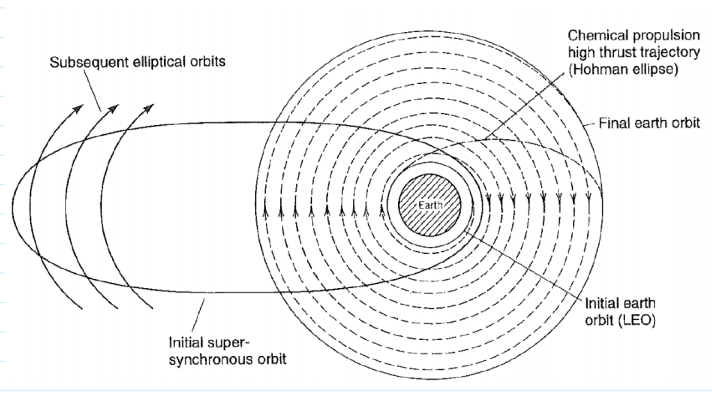
\includegraphics[scale=0.65]{1.png}
\newline \newline
\textbf{Side-Note:} Supersynchronous orbit: Spacecraft launched into very eccentric orbit with CP, supersynchronous elliptical orbit; from there electric propulsion can continuously and effectively be fired to attain a GEO orbit. Apogee $>$ GEO, EP used to circularize and reduce Apogee to GEO
\newline \newline
In 1961, Edelbaum solved this quasi-circular spiral trajectory problem, assuming quasi-circular spirals, apply a small inclination change per orbit.
\vfill
\begin{center}
\textbf{Figure 4}
\end{center}
\newpage
He also assumed optimum change in thrust angle, as the spacecraft spirals out, the thrust angle changes optimally.
\begin{shaded}
\textbf{Edelbaum Equation}
\begin{equation}
\Delta v = \sqrt{v_1^2 + v_2^2 - 2 v_1 v_2 \cos (\frac{\pi}{2} \theta)}
\end{equation}
Where:
\begin{equation*}
\begin{split}
\theta &= \text{Inclination Angle (in degrees)} \\
V_{\#} &= \text{Circular Orbit Velocity}\\
\end{split}
\end{equation*}
\end{shaded}
Before moving forward with the exercise, lets recall the definition and equations for a circular orbit velocity
\begin{shaded}
\textbf{Circular Orbit Velocity}
\begin{equation}
v_{\text{circular}} = \sqrt{\frac{\mu}{r}}
\end{equation}
Where:
\begin{equation*}
\begin{split}
\mu &= \text{Standard Gravitational Parameter} \\
& = G(M + m) \\
\mu_{\text{earth}} &= 3.986\text{x}10^{14} \frac{m^3}{s^2} \\
& = 3.986\text{x}10^{5} \frac{km^3}{s^2}\\
r &= \text{Radius of Orbit}\\
\end{split}
\end{equation*}
\end{shaded}
and an escape velocity.
\begin{shaded}
\textbf{Escape Velocity}
\begin{equation}
v_{\text{escape}} = \sqrt{2} v_{\text{circular}}
\end{equation}
\end{shaded}
\begin{center}
\vfill
\textbf{Figure 5}
\end{center}
\newpage
\begin{exer}
\textbf{
\\
Find the escape delta-V from LEO. Assume $v_1 = 7800 \frac{m}{s}$ orbital velocity} \\
\begin{itemize}
\item Chemical Propulsion: $\Delta V_{\text{chemical}}$
\begin{equation*}
\begin{align}
v_{\text{escape}} = \sqrt{2} 7800 = 11030 \frac{m}{s} \\
\Delta V_{\text{chemical}} = v_{\text{escape}}  - v_1 = 3230\frac{m}{s}
\end{align}
\end{equation*}
\item Electrical Propulsion: $\Delta V_{\text{electric}}$
\newline \newline
We will be using the Edelbaum equation for the case of Electric Propulsion. One thing to consider, since we are moving from LEO to an escaped path, our final orbit radius is $r = \infty$. \\
 \vspace{15mm}
\\
\begin{center}
\textbf{Figure 6}
\end{center}
As a result
\begin{equation*}
\begin{align}
v_{\text{circular}} &= 0 \quad \text{when r = 0}\\
v_1 &= 7800 \frac{m}{s} \\
v_2 &= 0\frac{m}{s} \\
\theta &= 0^{\circ} \text{, no inclination change}\\ \\
\text{Edelbaum Equation:}\\ \\
\Delta V_{\text{electrical}} &= \sqrt{7800^2 + 0^2 -0} = 7800 \frac{m}{s}
\end{align}
\end{equation*}
\end{itemize}
Note how $\Delta V_{\text{electric}}$ is higher! Why would we want to use it then? The reason is because it could have less propellant mass then chemical propulsion.
\newline
\newline
Consider the case where a chemical thruster and electric thruster use the same propellant mass. Then,
\begin{equation*}
\begin{align}
\frac{(I_{SP})_{\text{electric}}}{(I_{SP})_{\text{chemical}}} = \frac{\Delta V_{\text{electric}}}{\Delta V_{\text{chemical}}} = \frac{7800}{3230} = 2.4
\end{align}
\end{equation*}
\newline \newline
Therefore, we have to have 2.4 times more $I_{SP}$ for electric propulsion than chemical. If a typical chemical thruster has an $I_{SP} \approx 300\text{sec}$ then an electrical thruster must have $I_{SP} \approx 750\text{sec}$. Luckily, electric thrusters tend to range around $I_{SP} \approx 1000+\text{sec}$ meaning we most likely are saving on propellant mass.
\end{exer}
\newpage
\subsubsection{Power Supply Penalty}
The so-called "power supply penalty" places a premium on maximizing the specific power (in W/kg) of power supplies used for electric propulsion systems. Electric Propulsion has "massive" power generating system (PPU and Power Supply) and is low thrust, so its flight regime is much different than for chemical rockets. 
\newline \newline
The performance of the electric rocket can be analyzed in terms of the power and relevant masses.
\begin{shaded}
\textbf{Initial Mass Breakdown}
\begin{equation}
m_o = m_p + m_{pl} + m_{pp}
\end{equation}
Where:
\begin{equation*}
\begin{split}
m_{o} &= \text{Initial Mass} \\
m_{p} &= \text{Propellant Mass} \\
m_{pl} &= \text{Payload Mass} \\
m_{pp} &= \text{Power Plant Mass} \\
&= m_{\text{thruster}} + m_{\text{tank}} + m_{\text{feed system}} + m_{\text{PPU}} + m_{\text{power source}}
\end{split}
\end{equation*}
\end{shaded}
Let $\alpha$ be the mass specific power of the power plant, that is:
\begin{shaded}
\textbf{Specific Power}
\begin{equation}
\alpha = \frac{P}{m_{pp}} \quad \frac{\text{kW}}{\text{kg}}
\end{equation}
Where:
\begin{equation*}
\begin{split}
P &= \text{Electrical Power Output of the Power Plant with mass $m_{pp}$} \\
m_{pp} &= \text{Power Plant Mass} \\
\end{split}
\end{equation*}
\end{shaded}
Also (confusingly) $\alpha = \frac{m_{pp}}{P}\frac{\text{kg}}{\text{kW}}$ as seen in some cases like below. In class, we will most often use $\alpha$ as seen in Equation 17.
\newline
\newline
Typical $\alpha$ values:
\begin{itemize}
\item Very High Performance: $\alpha = 1 \frac{\text{kg}}{\text{kw}}$
\item High Performance:  $\alpha = 10 \frac{\text{kg}}{\text{kw}}$
\item Moderate Performance:  $\alpha = 30 \frac{\text{kg}}{\text{kw}}$
\item Low Performance: $\alpha = 100 \frac{\text{kg}}{\text{kw}}$
\end{itemize}

For Solar Electric Propulsion:
\begin{itemize}
\item Solar Panel: $150\frac{\text{W}}{\text{kg}} \rightarrow \alpha_{\text{electric}} = 6.7 \frac{\text{kg}}{\text{kw}}$
\item PPU:  $\alpha_{\text{PPU}} = 2.5 \frac{\text{kg}}{\text{kw}}$
\item Thruster, Mount, FeedSystem, Tank, etc:  $\alpha_{\text{t}} = 0.8 \frac{\text{kg}}{\text{kw}}$
\item Therefore... $\alpha_{\text{overall}} = 10 \frac{\text{kg}}{\text{kw}}$
\end{itemize}
Research is focused on achieving higher $\alpha$ values.
\newline \newline
The efficiency $\eta$ is 
\begin{framed}
\begin{equation}
\begin{aligned}
\eta = \frac{\frac{1}{2}Tc}{P} =  \frac{\frac{1}{2}\dot{m}c^{2}}{P}
\end{aligned}
\end{equation}
\end{framed}
Where c is the effective exhaust velocity and $\dot{m}$ is the mass flow rate. Then
\begin{equation*}
\begin{aligned}
m_{pp}=\frac{m_{p}c^{2}}{2\alpha t_t \eta} \qquad \qquad \dot{m} = \frac{m_p}{t_t}
\end{aligned}
\end{equation*}
Where $t_t$ is the burn or thrusting/propulsive time.
\newline \newline
Using Equation 12, the "Gravity-Free Rocket Equation", (no drag and no gravity so $\Delta V$ is simply the change in the velocity of the craft), where $m_f$ is the final mass 
\begin{equation*}
\begin{aligned}
\frac{m_o}{m_f} = \exp(\frac{\Delta V}{c}})
\end{aligned}
\end{equation*}
Where
\begin{equation*}
\begin{aligned}
m_{o} = m_{p} + m_{f} \qquad \text{ and }\qquad m_{f} = m_{pl} + m_{pp}
\end{aligned}
\end{equation*}
\newline
We will now begin to derive the payload mass fraction. \newline \newline
\textbf{Step 1:} Invert $\frac{m_o}{m_f}$
\begin{equation*}
\begin{aligned}
\frac{m_o}{m_f} = \exp(\frac{\Delta V}{c}) \qquad \rightarrow \qquad \frac{m_f}{m_o} = \exp(\frac{-\Delta V}{c})
\end{aligned}
\end{equation*}
\newline
\textbf{Step 2:} Substitute the equations for $m_f$ and $m_o$ 
\begin{equation*}
\begin{aligned}
m_o = m_{p} + m_f \qquad &\rightarrow \qquad m_f = m_{o} - m_{p} \\ \\
\frac{m_f}{m_o} = \frac{m_{o} - m_{p}}{m_o} &= 1 - \frac{m_p}{m_o} \\ \\ 
1 - \frac{m_p}{m_o} = \exp(\frac{-\Delta V}{c}) \qquad &\rightarrow \qquad  \frac{m_p}{m_o} = 1 - \exp (\frac{-\Delta V}{c}) \\ \\ 
\end{aligned}
\end{equation*}
\newline
\textbf{Step 3:} Do the same as in Step 2: this time for $\frac{m_{pl}}{m_o}$ 
\begin{equation*}
\begin{aligned}
\frac{m_f}{m_o} = \frac{m_{pl} + m_{pp}}{m_o} &= \frac{m_{pl}}{m_o} + \frac{m_{pp}}{m_o} \\ \\ 
 \frac{m_{pl}}{m_o} + \frac{m_{pp}}{m_o} = \exp(\frac{-\Delta V}{c}) \qquad &\rightarrow \qquad  \frac{m_{pl}}{m_o} = \exp(\frac{-\Delta V}{c}) - \frac{m_{pp}}{m_o}\\ \\ 
\end{aligned}
\end{equation*}
\textbf{Step 4:} Substitute $m_{pp}$ after making the correct simplifications.
\begin{equation*}
\begin{aligned}
m_{pp}=\frac{m_{p}c^{2}}{2\alpha t_t \eta}  \qquad &\rightarrow \qquad \frac{m_{pp}}{m_p}=\frac{c^{2}}{2\alpha t_t \eta} \\ \\ 
\frac{m_{pp}}{m_p}\frac{m_{p}}{m_o} = \frac{m_{pp}}{m_o} &=  \frac{c^{2}}{2\alpha t_t \eta}(1 - \exp (\frac{-\Delta V}{c}))\\ \\ 
\end{aligned}
\end{equation*}
\qquad \qquad $\frac{m_{pp}}{m_p}$ and  $\frac{m_{p}}{m_o}$ are known, therefore
\begin{equation*}
\begin{aligned}
\frac{m_{pl}}{m_o} &= \exp{\frac{-\Delta V}{c}} - \frac{m_{pp}}{m_o}
\end{aligned}
\end{equation*}
\newline
The resulting equation is known as the payload fraction. 
\begin{shaded}
\textbf{Payload Fraction}
\begin{equation*}
\frac{m_{pl}}{m_o} = \exp{\frac{-\Delta V}{c}} - \frac{c^{2}}{2\alpha t_t \eta}(1 - \exp (\frac{-\Delta V}{c}))
\end{equation*}
\end{shaded}
\newline
We can define a "characteristic speed" or "characteristic velocity" as Stuhlinger [1964] and Irving [1959] did.
\begin{shaded}
\textbf{Characteristic Speed}
\begin{equation}
v_c = \sqrt{2 \alpha \eta t_t}
\end{equation}
\end{shaded}
It has no physical meaning but represents the speed that the power plant mass $m_{pp}$ would have if its full power output were converted to kinetic energy of its own mass. With the characteristic speed, we can take the inverse and rewrite our Payload Fraction as
\begin{shaded}
\textbf{Payload Fraction (Inverted; In terms of Characteristic Speed)}
\begin{equation}
\frac{m_{o}}{m_{pl}} = \frac{\exp{\frac{\Delta V}{c}}}{1 - (\exp (\frac{\Delta V}{c})-1)\frac{c^{2}}{v_{c}^{2}}}
\end{equation}
Here we see the payload ration in terms of the power-plant properties! We typically want the $\frac{m_{pl}}{m_{o}}$ value to be high because we want to transport more cargo.
\end{shaded}
A plot of $\frac{m_{pl}}{m_{o}}$ for $\frac{c}{v_c}$ is shown below. 
\newline
\begin{center}
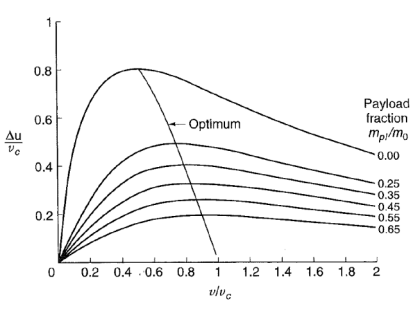
\includegraphics[scale=0.75]{2.png}
\end{center}
\begin{itemize}
\item For a given payload fraction there is an optimum value of c ($I_{SP}$) corresponding to the most delta-V.
\item Peaks exists cause $m_{pp}$ increases with $I_{SP}$ (commonly called the "power supply penalty") but $m_p$ decreases with $I_{SP}$.
\item For a given mission (delta-V) there exists a theoretical optimum range of $I_{SP}$ and thus optimum propulsion system.
\item Peaks are for
\begin{equation*}
\begin{align}
\frac{\Delta V}{V_{c}} \leq 0.805 \qquad \text{and} \qquad 0.805 < \frac{c}{V_{c}} < 1.0
\end{align}
\end{equation*}
\begin{itemize}
\item $\Delta v \propto v_c \rightarrow \Delta v^2 \propto t_t$: Optimum operating time is proportional to $\Delta v^2$. As a result $t_t$ is long for large $\Delta v$.
\item $\Delta v \propto v_c$ with $c \propto v_c$, so $\Delta v \propto c$ and $c \propto I_{SP}$. Optimum $I_{SP} \propto \Delta v$, therefore large $\Delta v$ requires large $I_{SP}$.
\end{itemize}
\end{itemize}
The peak of the curves can be found by differentiating Equation 20. The following equation gives the optimum c for a given delta-V and characteristic speed $v_c$.
\begin{shaded}
\textbf{Payload Fraction Peaks: Optimum Line Equation}
\begin{equation}
\frac{c}{\Delta V}(\exp (\frac{\Delta V}{c})-1)-\frac{1}{2}(\frac{v_c}{c})^{2}-\frac{1}{2} = 0
\end{equation}
\end{shaded}
Another way to look at this tradeoff between power supply mass and propellant mass is....
\begin{equation*}
\begin{aligned}
m_p &= \dot{m}t_t \qquad \text{(Equation 2)}\\ \\
T &= \dot{m} c \\ \\
&\rightarrow m_p = \frac{T t_t}{c} \qquad \text{Substitute with Equation 3}
\end{aligned}
\end{equation*}
\begin{equation}
\begin{aligned}
\rightarrow \qquad m_p = \frac{T t_t}{g I_{SP}} \propto \frac{1}{I_{SP}}
\end{aligned}
\end{equation}
\newline
Now we want to use the least amount of $m_p$ so we want a large $I_{SP}$. BUT power supply
penalty, using Equation 17, $\frac{\text{Equation 7}}{\text{Equation 18}}$ and Equation 3 we arrive at:
\newline
\begin{equation}
\begin{aligned}
m_{pp} = \frac{P}{\alpha} = \frac{T c}{2 \eta \alpha} = \frac{T g}{2 \eta \alpha}I_{SP} \propto I_{SP}
\end{aligned}
\end{equation}
\newline
If we have large $I_{SP}$, then we must have a large power plant to carry along. There must be an optimum! \textbf{Optimum = least propellant AND power supply mass.}
\begin{center}
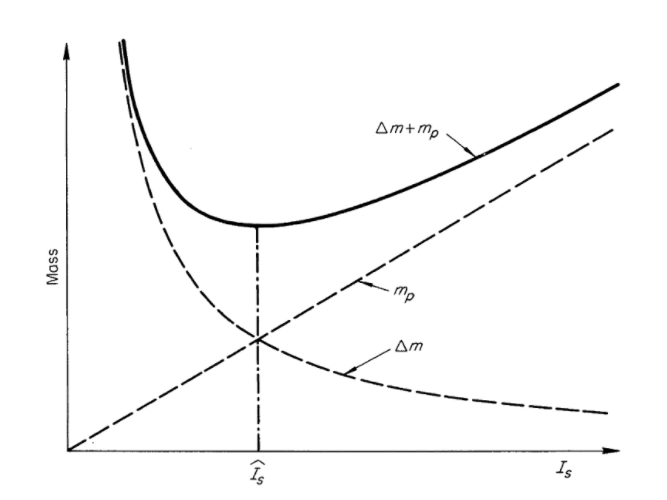
\includegraphics[scale=0.5]{5.png}
\end{center}
\begin{equation*}
\begin{aligned}
\frac{\partial (m_p + m_{pp})}{\partial (gI_{SP})} = 0 = \frac{-T t_t}{(g I_{SP})^2}+\frac{T}{2 \eta \alpha}
\end{aligned}
\end{equation*}
Which gives us
\begin{shaded}
\textbf{Optimum c for Minimum Mass}
\begin{equation}
\begin{aligned}
(g I_{SP})_{\text{optimum}} = \sqrt{2 \eta \alpha t_t} = v_c = c
\end{aligned}
\end{equation}
\end{shaded}
\newline
Equation 21 gives us the optimum c for a max delta-V because there is no linear relation between mass and delta-V (ln relation). Equation 24 gives us the optimum c for minimum mass.
\newpage
\subsubsection{Spacecraft Design Procedure}
Given the payload mass, $m_pl$, and vehicle velocity increment, (delta-V), a spacecraft design procedure could proceed as:
\begin{enumerate}
\item Pick an arbitrary payload mass fraction ($\frac{m_{pl}}{m_o}) \quad \rightarrow \quad$ which would yield an optimum $\frac{\Delta v}{v_c}$ either from the figure or Equation 21
\item From the given $\Delta v$  determine $v_c$ from Equation 21
\item From optimum $\frac{c}{v_c}$ at given payload mass fraction (Equation 21), determine corresponding c and $I_{SP}$.
\item Select an engine that can deliver this optimum $I_{SP}$ (and from the thruster's $\alpha$ and $\eta$) find the thrusting time $t_t$ alongside Equation 19, with $v_c$
\item Calculate the propellant mass, $m_p$, using the rocket equation (Equation 12) and your picked payload ratio (your guess/pick in step 1)
\item Check that vehicle electrical power, volume, mass, and mission time are not exceeded. In other words, reconcile the results from Steps 1-5 with the other spacecraft design parameters (e.g., available power, mass, volume, mission time). Will it fit within the spacecraft and mission constraints? If...
\begin{itemize}
\item \textbf{Yes}, Awesome!
\item \textbf{No}, go back to step 1with lower payload ratio.
\end{itemize}
\end{enumerate}
As noted in step 1, there is no unique criterion for selecting payload mass fraction. We simply pick and hope the resulting mass, volume, power requirements can be met.
\newline \newline
More sophisticated approaches use a "dual optimum" technique where they optimize by seeking shortest burn time with the highest payload mass fraction for the vehicle. How doe we optimize time and payload ration? By using transfer rates!
\newpage
\subsubsection{Transfer Rate}
What about $t_t$? We said at beginning of Section I.6. that for a space mission design, we need to know $\Delta v$ and $t_t$. Only then can we calculate $\frac{m_{pl}}{m_o}$.
\newline
\begin{framed}
\textbf{Side Note:}
\newline
For some missions, electric propulsion may get to GEO sooner and cost less, when one considers the entire spacecraft and launch vehicle timeline
\begin{center}
\vspace{30mm}
\textbf{Figure 6}
\end{center}
\end{framed}
But back to the spacecraft mission in space. How can we determine $t_t$? (How do we minimize the time required?)
\newline \newline
One way to resolve $t_t$ is to treat it as a variable. We did not do this previously. Previously we found an optimum c (or $I_{SP}$) to either
\begin{itemize}
\item minimize mass $m_{p} + m_{pp}$ , given $\eta$ , $\alpha$ , $t_t$. This was Equation 25.
\item maximize payload ratio, given $\eta$ , $\alpha$ , $t_t$. This was Equation 21.
\end{itemize}
Now, we treat $t_t$ as a variable, and search for a "dual" optimum, we want to transfer the most payload in the shortest time. \textbf{Maximize $m_{pl}$ while Minimizing $t_t$.}
\newline
\begin{equation*}
\begin{aligned}
m_{pl} &= m_o - m_p - m_{pp} & \qquad \text{Equation 16} \\
\frac{m_{p}}{m_o} &= 1 - \exp [\frac{-\Delta V}{c}]\\
\frac{m_{pp}}{m_o} &=  \frac{T c}{2 \eta \alpha m_o} & \qquad \text{Equation 23} \\
\end{aligned}
\end{equation*}
\begin{framed}
\begin{equation}
\begin{aligned}
\frac{m_{pl}}{m_o} = \exp [\frac{-\Delta V}{c}] - \frac{T c}{2 \eta \alpha m_o}\\
\end{aligned}
\end{equation}
\end{framed}
\begin{shaded}
\textbf{Transfer Rate}
\begin{equation}
\begin{aligned}
\text{TR} = \frac{\frac{m_{pl}}{m_o}}{t_t}
\end{aligned}
\end{equation}
\end{shaded}
\newline
From Pukniel and Burton, Journals Spacecraft and Rockets, Vol 45, No1, 2008. For a LEO$\rightarrow$ GEO $\rightarrow$ LEO returning SpaceTug. For fixed $\eta$, $\alpha$, P, T:
\newline
\begin{framed}
\begin{equation}
\begin{aligned}
\frac{(\Delta v)^{2} \text{TR}}{2 \alpha \eta} = (\frac{m_{pp}}{m_o})(\frac{\Delta v}{c})^2 \frac{\exp[\frac{-\Delta v}{c}] - (\frac{m_{pp}}{m_o})\exp[\frac{\Delta v}{c}]}{1-\exp[\frac{-\Delta v}{c}]+(\frac{m_{pp}}{m_o})(\exp[\frac{\Delta v}{c}]-1)}
\end{aligned}
\end{equation}
\newline
\end{framed}
\newline
A plot of Equation 27 shows...
\newline
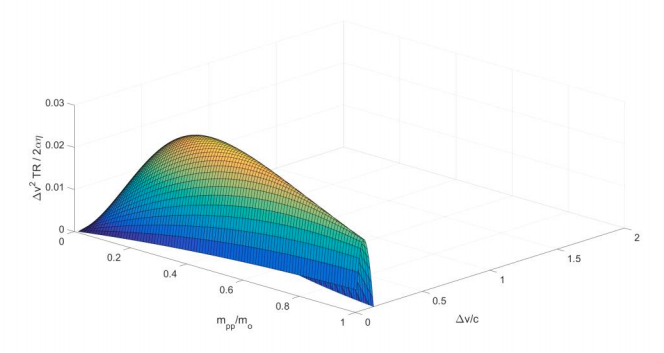
\includegraphics[scale=0.75]{3.png}
\newline \newline
a maximum.
\newline
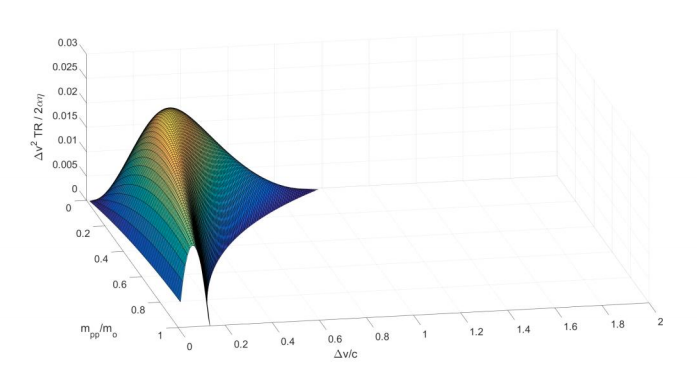
\includegraphics[scale=0.75]{4.png}
\newline \newline
Optimum is at..
\newline
\begin{equation*}
\begin{aligned}
\frac{m_{pp}}{m_{o}}= 18.5\% \qquad 
\frac{m_{p}}{m_{o}}= 45\% \qquad 
\frac{m_{pl}}{m_{o}}= 36.5\% \qquad 
\frac{\Delta v}{c}= 0.43 \qquad 
\frac{(\Delta v)^{2} \text{TR}}{2 \alpha \eta} = 0.0279
\end{aligned}
\end{equation*}
\newline \newline
\textbf{Summary:} There are many ways to optimize an electric spacecraft 
\newline
\newline
\textbf{Optimization Gives:}  $I_{SP}$, $\frac{m_{p}}{m_o}$, $\frac{m_{pp}}{m_o}$, $t_t$
\newline
\newline
Now we know the parameters for which to select the "best" thruster for a particular mission. Moving forward we need to know about the different types of electric propulsion thrusters, but first we need to review Electromagnetics. 
 
\end{document}